\documentclass[11pt,a4paper]{article}

% ── Packages ──────────────────────────────────────────────────────────────────
\usepackage[utf8]{inputenc}
\usepackage[T1]{fontenc}
\usepackage{amsmath,amssymb}
\usepackage{graphicx}
\usepackage{booktabs}
\usepackage{hyperref}
\usepackage{cleveref}
\usepackage{algorithm}
\usepackage{algorithmic}
\usepackage{tikz}
\usetikzlibrary{automata,positioning,arrows.meta,fit,backgrounds}
\usepackage{subcaption}
\usepackage{enumitem}
\usepackage{xcolor}
\usepackage{natbib}
\usepackage[margin=1in]{geometry}
\usepackage{microtype}

% ── Metadata ──────────────────────────────────────────────────────────────────
\title{Agentic Conversation for Action: A Recursive State Machine\\for Intent-Aligned Multi-Agent Coordination\\with Backtracking and Human Proxy}

\author{Darrell Pinto}

\date{March 2026}

% ══════════════════════════════════════════════════════════════════════════════
\begin{document}
\maketitle

% ── Abstract ──────────────────────────────────────────────────────────────────
\begin{abstract}
Large language model (LLM) agents increasingly operate in multi-step,
multi-agent workflows where the gap between human intent and agent execution
produces costly misalignment. We present \emph{Agentic Conversation for Action}
(Agentic CfA), a recursive three-phase state machine---Intent Alignment,
Planning, and Execution---that extends the classical Conversation for Action
framework of Winograd and Flores to autonomous agent coordination. Three
architectural contributions distinguish this work from prior agent
orchestration approaches. First, an explicit \emph{intent alignment phase}
produces a governing intent document through structured human--agent dialog
before any planning or execution begins, addressing the root cause of
misalignment rather than its symptoms. Second, \emph{cross-phase backtracking}
allows execution-time discoveries to trigger re-entry into planning or intent
alignment without restarting the workflow, enabling the system to correct
upstream assumptions at the moment they are falsified. Third, a \emph{human
proxy} with a learned confidence model replaces the binary choice between full
human oversight and full autonomy: the proxy auto-approves decisions where its
learned model of human preferences is confident, and escalates to the human
otherwise, with cold-start safeguards, staleness guards, exploration sampling,
and asymmetric regret weighting that make false approvals harder to earn than
false escalations. We describe the formal state machine (18 states, 40+
transitions across three phases), the confidence-based approval gate, the
hierarchical memory and learning system, and a reference implementation built
on Claude Code CLI. Empirical observations from production sessions
demonstrate that the architecture reduces rework, enables earned autonomy, and
maintains alignment across hierarchical agent teams without prescriptive prompt
engineering.
\end{abstract}

\noindent\textbf{Keywords:} multi-agent systems, human--AI alignment, conversation for action, state machines, intent engineering, human-in-the-loop, confidence calibration, LLM agents

% ══════════════════════════════════════════════════════════════════════════════
\section{Introduction}
\label{sec:introduction}

The dominant paradigm for LLM-based agent systems follows a plan--execute
model: the human provides a request, the agent plans how to fulfill it, then
executes. This model fails in proportion to the gap between what the human
\emph{said} and what the human \emph{meant}. That gap contains organizational
values, unstated tradeoffs, decision boundaries, domain constraints, and
quality expectations that the human has internalized to the point of
invisibility.

Prompt engineering tells agents \emph{what to do}. Context engineering tells
agents \emph{what to know}. Neither addresses the deeper question: what should
the agent \emph{want}---what to optimize for, what to protect, and what
tradeoffs are acceptable? We call this missing layer \emph{intent engineering},
and its absence is the structural root of agent misalignment in production
systems.

The consequences are well-documented. An AI system deployed to reduce costs
may optimize the metric while destroying the organizational relationships that
produce long-term value. Code that passes every test may miss the actual use
case. A report that fulfills all stated requirements may answer questions the
reader was not asking. In each case, the agent did what it was told; the
problem is that what it was told was an incomplete specification of what was
wanted.

This paper presents \emph{Agentic Conversation for Action} (Agentic CfA), an
architecture that addresses intent misalignment structurally rather than
through better prompting. The framework makes three contributions:

\begin{enumerate}[label=(\arabic*)]
    \item \textbf{Intent Alignment Phase.} Before any planning or execution,
    a structured dialog between human and agent produces a governing intent
    document (INTENT.md) that captures not just what to build but \emph{why},
    with explicit success criteria, decision boundaries, escalation posture,
    and constraints. This phase is the architectural recognition that alignment
    is a conversation, not a specification.

    \item \textbf{Cross-Phase Backtracking.} The state machine supports
    transitions that re-enter earlier phases---from execution back to planning,
    or from planning back to intent alignment---at synthesis points rather than
    decision points. This allows the system to correct upstream assumptions at
    the moment they are falsified, rather than completing misaligned work and
    extracting post-hoc learnings.

    \item \textbf{Human Proxy with Learned Confidence.} A confidence-based
    approval gate replaces the binary choice between human-in-the-loop and
    full autonomy. The proxy learns from human approval and correction
    patterns, auto-approving when its model is confident and escalating
    otherwise. Cold-start safeguards, staleness guards, exploration sampling,
    and asymmetric regret weighting ensure that autonomy is earned through
    demonstrated alignment, not granted by configuration.
\end{enumerate}

The architecture is grounded in Winograd and Flores's Conversation for Action
(CfA) framework \citep{winograd1986understanding}, which models collaborative
work as structured conversations with explicit commitments, breakdowns, and
renegotiations. We extend this framework from dyadic human interaction to
multi-agent hierarchical teams, adding recursive phase structure and learned
autonomy progression.

\Cref{sec:related} reviews related work.
\Cref{sec:framework} presents the formal CfA state machine.
\Cref{sec:intent} describes the intent alignment phase.
\Cref{sec:proxy} details the human proxy and confidence model.
\Cref{sec:backtracking} analyzes cross-phase backtracking.
\Cref{sec:learning} presents the learning and memory system.
\Cref{sec:implementation} describes the reference implementation.
\Cref{sec:evaluation} reports empirical observations.
\Cref{sec:discussion} discusses implications and limitations.
\Cref{sec:conclusion} concludes.

% ══════════════════════════════════════════════════════════════════════════════
\section{Related Work}
\label{sec:related}

\subsection{Conversation for Action}

The Conversation for Action framework \citep{winograd1986understanding}
models human collaboration as structured speech acts with explicit states:
request, promise, report completion, declaration of satisfaction or
breakdown. The framework was influential in computer-supported cooperative
work (CSCW), notably through the Coordinator system
\citep{flores1988computer}, but was criticized for rigidity when applied to
human workflow management \citep{suchman1994plans}. We argue that the
properties that made CfA awkward for human workflows---explicit state,
formal transitions, verifiable commitments---make it well-suited for
agent coordination, where implicit social negotiation is unavailable and
explicit protocol is necessary.

\subsection{Cognitive Architectures for Language Agents}

The CoALA framework \citep{sumers2024cognitive} provides a unifying taxonomy
mapping classical cognitive architectures onto LLM agents, distinguishing
memory types (episodic, semantic, procedural), action spaces, and learning
mechanisms. Our learning system (\Cref{sec:learning}) adopts CoALA's
memory taxonomy while adding scope-differentiated retrieval and a promotion
chain that filters learnings as they propagate through hierarchical levels.

\subsection{Multi-Agent Coordination}

Recent work on multi-agent LLM systems includes
AutoGen \citep{wu2023autogen}, which provides a framework for conversational
agents with human participation;
MetaGPT \citep{hong2023metagpt}, which assigns software engineering roles to
agents with structured output schemas; and
ChatDev \citep{qian2024chatdev}, which simulates software companies with
role-playing agents. These systems coordinate agents through role-playing and
conversational protocols but lack formal state machines, cross-phase
backtracking, or learned autonomy progression. Our work differs in providing
a formal coordination protocol with verifiable state transitions and
a human proxy that learns approval patterns over time.

\subsection{Learning from Interaction}

Several approaches enable LLM agents to learn from experience without
weight updates. Reflexion \citep{shinn2023reflexion} uses verbal
self-reflection stored as persistent memory.
CLIN \citep{majumder2024clin} learns causal abstractions that persist
across episodes and transfer across tasks.
ExpeL \citep{zhao2024expel} extracts cross-task insights from contrastive
analysis of successes and failures.
Generative Agents \citep{park2023generative} use three-factor retrieval
(recency, relevance, importance) with periodic reflection. Our learning
system draws on these approaches while adding scope-differentiated
storage, confidence-weighted decay, and a hierarchical promotion chain.

\subsection{Human-in-the-Loop Agent Systems}

The tension between human oversight and agent autonomy is central to
deployable agent systems. Inner Monologue \citep{huang2023inner} uses
human feedback as environment grounding for embodied agents.
MemGPT \citep{packer2023memgpt} gives agents explicit memory management
tools, enabling them to decide what to remember and retrieve. Our human
proxy differs from these approaches by learning \emph{when} human input
is needed rather than \emph{what} to ask, framing the problem as
confidence calibration rather than information gathering.

\subsection{Shared Mental Models in Human--AI Teaming}

Research on shared mental models (SMMs) in organizational psychology
\citep{cannon2001work} demonstrates that team performance depends not on
shared information but on shared \emph{interpretation} of that information.
High-performing teams can anticipate each other's actions and make locally
good decisions that are globally coherent. Our intent alignment phase
(\Cref{sec:intent}) is designed to produce an SMM between human and agent,
and the human proxy (\Cref{sec:proxy}) operationalizes the trust-building
process that organizational psychology research identifies as incremental
and asymmetric \citep{edmondson1999psychological}.

% ══════════════════════════════════════════════════════════════════════════════
\section{The Agentic CfA Framework}
\label{sec:framework}

\subsection{Overview}

Agentic CfA is a recursive three-phase state machine that governs the
lifecycle of a unit of work from initial idea to completed deliverable.
The three phases are:

\begin{description}[style=nextline]
    \item[Phase 1: Intent Alignment (IDEA $\to$ INTENT)]
    Produce a governing intent document capturing what the human wants,
    why it matters, what success looks like, and where agent autonomy
    begins and ends.

    \item[Phase 2: Planning (INTENT $\to$ PLAN)]
    Given approved intent, produce an implementation plan that
    decomposes intent into actionable tasks while preserving alignment
    with the original purpose.

    \item[Phase 3: Execution (PLAN $\to$ COMPLETED\_WORK)]
    Execute the plan, deliver completed work, and handle the
    inevitable discoveries that execution produces.
\end{description}

Each phase contains states for normal progression, human interaction
(questions, escalations, assertions), and backtracking to earlier phases.
The full state machine comprises 18 states and over 40 valid transitions.

\subsection{Formal State Machine}

We define the CfA state machine as a tuple $\mathcal{M} = (S, A, \delta, s_0, F)$ where:

\begin{itemize}
    \item $S$ is the set of states, partitioned into intent states $S_I$,
    planning states $S_P$, and execution states $S_E$:
    \begin{align*}
        S_I &= \{\text{IDEA}, \text{PROPOSAL}, \text{INTENT\_QUESTION}, \\
            &\quad\;\; \text{INTENT\_ESCALATE}, \text{INTENT\_ASSERT}, \\
            &\quad\;\; \text{INTENT\_RESPONSE}, \text{INTENT}\} \\
        S_P &= \{\text{DRAFT}, \text{PLANNING\_QUESTION}, \\
            &\quad\;\; \text{PLANNING\_ESCALATE}, \text{PLAN\_ASSERT}, \\
            &\quad\;\; \text{PLANNING\_RESPONSE}, \text{PLAN}\} \\
        S_E &= \{\text{TASK}, \text{TASK\_IN\_PROGRESS}, \\
            &\quad\;\; \text{TASK\_QUESTION}, \text{TASK\_ESCALATE}, \\
            &\quad\;\; \text{TASK\_ASSERT}, \text{TASK\_RESPONSE}, \\
            &\quad\;\; \text{FAILED\_TASK}, \text{COMPLETED\_TASK}, \\
            &\quad\;\; \text{WORK\_IN\_PROGRESS}, \text{WORK\_ASSERT}, \\
            &\quad\;\; \text{COMPLETED\_WORK}, \text{WITHDRAWN}\}
    \end{align*}

    \item $A$ is the set of actions (transition labels): \texttt{propose},
    \texttt{question}, \texttt{escalate}, \texttt{assert},
    \texttt{auto-approve}, \texttt{answer}, \texttt{clarify},
    \texttt{approve}, \texttt{correct}, \texttt{withdraw},
    \texttt{synthesize}, \texttt{plan}, \texttt{delegate},
    \texttt{accept}, \texttt{failed}, \texttt{retry},
    \texttt{refine-intent}, \texttt{revise-plan}, \texttt{backtrack}.

    \item $\delta: S \times A \rightharpoonup S$ is the (partial) transition
    function. Each transition is additionally annotated with an \emph{actor}
    constraint specifying which role may take the action (human, intent\_team,
    planning\_team, execution\_worker, execution\_lead, research\_team,
    approval\_gate).

    \item $s_0 = \text{IDEA}$ is the initial state.

    \item $F = \{\text{COMPLETED\_WORK}, \text{WITHDRAWN}\}$ is the set of
    terminal states.
\end{itemize}

\subsection{Phase Structure}

Each phase follows a common pattern with role-specific variations:

\begin{enumerate}
    \item \textbf{Proposal/Draft/Task}: An agent produces an initial artifact.
    \item \textbf{Question}: The agent identifies a gap requiring research (routed to research team).
    \item \textbf{Escalation}: The agent identifies a gap requiring human judgment.
    \item \textbf{Assertion}: The agent asserts the artifact is ready for approval.
    \item \textbf{Response}: Feedback (from research, human, or lead) is synthesized.
    \item \textbf{Terminal}: The phase-terminal state (INTENT, PLAN, COMPLETED\_WORK) marks approval.
\end{enumerate}

The Question $\to$ Response $\to$ Synthesis loop can iterate multiple
times within a phase, allowing the agent to progressively refine its
artifact through research and feedback before asserting readiness.

\subsection{State Machine Diagram}

\begin{figure}[ht]
\centering
\resizebox{\textwidth}{!}{%
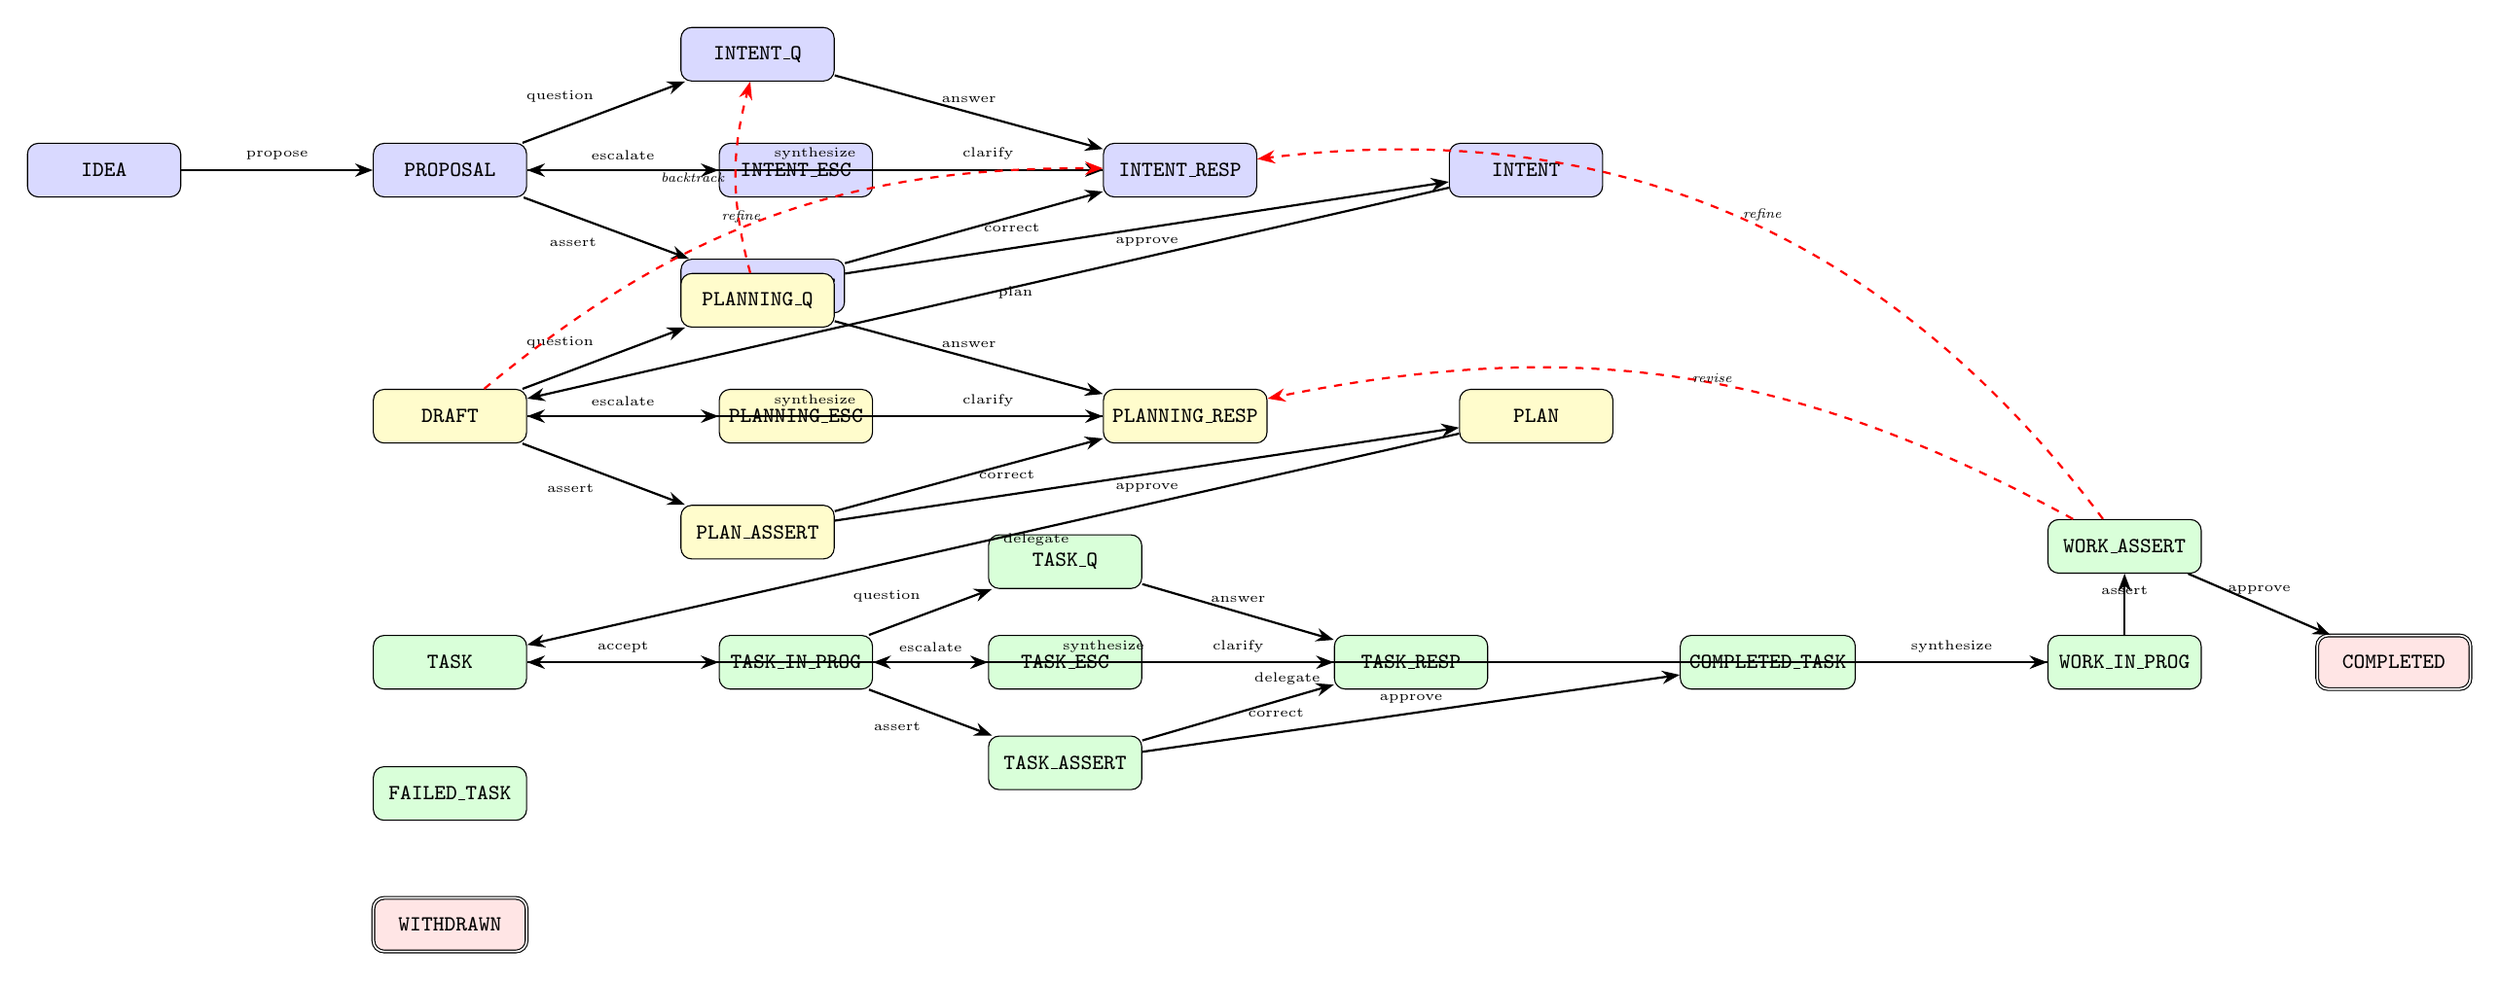
\begin{tikzpicture}[
    >=Stealth,
    node distance=1.8cm and 2.5cm,
    state/.style={
        rectangle, rounded corners, draw, minimum width=2cm,
        minimum height=0.7cm, font=\footnotesize\ttfamily,
        text centered
    },
    intent/.style={state, fill=blue!15},
    planning/.style={state, fill=yellow!20},
    execution/.style={state, fill=green!15},
    terminal/.style={state, fill=red!10, double},
    edge/.style={->, thick, font=\tiny},
    backtrack/.style={->, thick, dashed, red, font=\tiny},
]

% Intent phase
\node[intent] (idea) {IDEA};
\node[intent, right=of idea] (proposal) {PROPOSAL};
\node[intent, above right=0.8cm and 2cm of proposal] (iq) {INTENT\_Q};
\node[intent, right=of proposal] (ie) {INTENT\_ESC};
\node[intent, below right=0.8cm and 2cm of proposal] (ia) {INTENT\_ASSERT};
\node[intent, right=3cm of ie] (ir) {INTENT\_RESP};
\node[intent, right=of ir] (intent) {INTENT};

% Planning phase
\node[planning, below=2.5cm of proposal] (draft) {DRAFT};
\node[planning, above right=0.8cm and 2cm of draft] (pq) {PLANNING\_Q};
\node[planning, right=of draft] (pe) {PLANNING\_ESC};
\node[planning, below right=0.8cm and 2cm of draft] (pa) {PLAN\_ASSERT};
\node[planning, right=3cm of pe] (pr) {PLANNING\_RESP};
\node[planning, right=of pr] (plan) {PLAN};

% Execution phase
\node[execution, below=2.5cm of draft] (task) {TASK};
\node[execution, right=of task] (tip) {TASK\_IN\_PROG};
\node[execution, above right=0.6cm and 1.5cm of tip] (tq) {TASK\_Q};
\node[execution, right=1.5cm of tip] (te) {TASK\_ESC};
\node[execution, below right=0.6cm and 1.5cm of tip] (tass) {TASK\_ASSERT};
\node[execution, right=2.5cm of te] (tr) {TASK\_RESP};
\node[execution, below=1cm of task] (ft) {FAILED\_TASK};
\node[execution, right=of tr] (ct) {COMPLETED\_TASK};
\node[execution, right=of ct] (wip) {WORK\_IN\_PROG};
\node[execution, above=0.8cm of wip] (wa) {WORK\_ASSERT};
\node[terminal, right=1.5cm of wip] (cw) {COMPLETED};
\node[terminal, below=1cm of ft] (wd) {WITHDRAWN};

% Intent edges
\draw[edge] (idea) -- node[above] {propose} (proposal);
\draw[edge] (proposal) -- node[above left] {question} (iq);
\draw[edge] (proposal) -- node[above] {escalate} (ie);
\draw[edge] (proposal) -- node[below left] {assert} (ia);
\draw[edge] (iq) -- node[above] {answer} (ir);
\draw[edge] (ie) -- node[above] {clarify} (ir);
\draw[edge] (ia) -- node[below] {approve} (intent);
\draw[edge] (ia) -- node[right] {correct} (ir);
\draw[edge] (ir) -- node[above] {synthesize} (proposal);

% Intent to Planning
\draw[edge] (intent) -- node[right] {plan} (draft);

% Planning edges
\draw[edge] (draft) -- node[above left] {question} (pq);
\draw[edge] (draft) -- node[above] {escalate} (pe);
\draw[edge] (draft) -- node[below left] {assert} (pa);
\draw[edge] (pq) -- node[above] {answer} (pr);
\draw[edge] (pe) -- node[above] {clarify} (pr);
\draw[edge] (pa) -- node[below] {approve} (plan);
\draw[edge] (pa) -- node[right] {correct} (pr);
\draw[edge] (pr) -- node[above] {synthesize} (draft);

% Planning to Execution
\draw[edge] (plan) -- node[right] {delegate} (task);

% Execution edges
\draw[edge] (task) -- node[above] {accept} (tip);
\draw[edge] (tip) -- node[above left] {question} (tq);
\draw[edge] (tip) -- node[above] {escalate} (te);
\draw[edge] (tip) -- node[below left] {assert} (tass);
\draw[edge] (tq) -- node[above] {answer} (tr);
\draw[edge] (te) -- node[above] {clarify} (tr);
\draw[edge] (tass) -- node[above] {approve} (ct);
\draw[edge] (tass) -- node[right] {correct} (tr);
\draw[edge] (tr) -- node[above] {synthesize} (tip);
\draw[edge] (ct) -- node[above] {synthesize} (wip);
\draw[edge] (wip) -- node[above] {assert} (wa);
\draw[edge] (wa) -- node[above] {approve} (cw);
\draw[edge] (wip) -- node[below] {delegate} (task);

% Backtracking
\draw[backtrack, bend left=20] (draft) to node[left, text=black] {\textit{refine}} (ir);
\draw[backtrack, bend left=15] (pq) to node[left, text=black] {\textit{backtrack}} (iq);
\draw[backtrack, bend right=20] (wa) to node[right, text=black] {\textit{revise}} (pr);
\draw[backtrack, bend right=30] (wa) to node[right, text=black] {\textit{refine}} (ir);

\end{tikzpicture}
}
\caption{Agentic CfA state machine (simplified). Solid arrows show forward
transitions; dashed red arrows show cross-phase backtracking. States are
colored by phase: blue (intent), yellow (planning), green (execution).
Terminal states shown with double borders.}
\label{fig:state-machine}
\end{figure}

% ══════════════════════════════════════════════════════════════════════════════
\section{Intent Alignment Phase}
\label{sec:intent}

\subsection{The Intent Gap}

The fundamental challenge in agent orchestration is not execution quality
but specification quality. We define the \emph{intent gap} as the
information lost when human intent is compressed into an actionable
request. This gap contains:

\begin{itemize}
    \item \textbf{Purpose}: why the task matters to the organization,
    not just what artifact to produce.
    \item \textbf{Qualitative criteria}: values, style, and ``feel''
    that cannot be expressed as measurable thresholds.
    \item \textbf{Decision boundaries}: where agent autonomy begins
    and ends for this specific task.
    \item \textbf{Implicit constraints}: organizational, temporal, and
    resource boundaries the human has internalized.
    \item \textbf{Tradeoff preferences}: which competing values take
    priority when they conflict.
\end{itemize}

The intent alignment phase exists to close this gap through structured
dialog before any planning or execution begins.

\subsection{INTENT.md as Shared Mental Model}

The output of the intent alignment phase is a prose document
(INTENT.md) that serves as the governing specification for all
downstream work. Drawing on organizational psychology research on
shared mental models \citep{cannon2001work}, we design INTENT.md not
as a requirements document but as an artifact of shared understanding.

The quality criterion is not formal completeness but alignment:
\emph{does an agent reading this document develop a mental model
that matches the human's?} A formally complete document that leaves
genuine ambiguity about decision authority or tradeoff preferences
has failed. A concise document that creates genuine alignment has
succeeded.

Five types of content must be present:

\begin{enumerate}
    \item \textbf{Objective}: the outcome the human wants and why it
    matters---not the task, but the purpose the task serves.
    \item \textbf{Success criteria}: both quantitative (measurable
    thresholds) and qualitative (values, feel, style). Qualitative
    criteria are first-class, not a lesser version of quantitative ones.
    \item \textbf{Decision boundaries and escalation posture}: where
    the agent should use its judgment, where it should consult the
    human, and what it must never do.
    \item \textbf{Constraints}: technical, organizational, temporal,
    and resource boundaries.
    \item \textbf{Open questions}: ambiguities that cannot be resolved
    during intent gathering, which the planning phase must actively
    research and resolve.
\end{enumerate}

\subsection{Dialog Protocol}

The intent gathering conversation follows three governing principles:

\begin{description}
    \item[Every sentence must earn its place.] If removing a sentence
    would not change the reader's ability to understand the intent,
    remove it.
    \item[The reasonable person test.] Read every artifact as someone
    who was not in the room. If they cannot proceed with what they
    have been given, the document is incomplete.
    \item[Bring solutions, not questions.] The agent researches the
    problem space and presents alternatives with recommendations,
    rather than asking open-ended questions that transfer cognitive
    burden to the human.
\end{description}

The protocol distinguishes \emph{cold start} (no prior context) from
\emph{warm start} (accumulated institutional memory). In cold start,
the human is the sole source of intent and the agent conducts responsive
dialog that surfaces implicit assumptions. In warm start, the agent
pre-populates intent elements from prior interactions, presenting them
for confirmation rather than silently assuming them. The warm-start
protocol reduces human burden as the system matures, with corrections
to pre-populated elements treated as high-value calibration signals.

The conversation is constrained to 15 minutes for moderate-complexity
projects, with a maximum of 10 rounds and 30 total turns. These
constraints are design choices, not limitations: they force concision
and prevent the intent phase from becoming an open-ended requirements
elicitation process.

\subsection{Least-Regret Escalation}

Every autonomous agent faces a continuous choice: act or ask. Both
carry risk. Acting when the human wanted to be consulted causes wrong
work and eroded trust. Escalating when the agent could have handled
it wastes human attention and fails to deliver on the promise of
autonomy. These failure modes are asymmetric: their relative costs
vary by organization, individual, domain, and specific decision.

We formalize this as a \emph{least-regret} decision: the agent should
choose the option with the lowest expected regret, requiring three
capabilities:

\begin{enumerate}
    \item A \emph{model of human risk tolerance}, learned from
    observing human reactions over time.
    \item A \emph{model of action cost}: how reversible is the
    decision, and how much organizational impact does it carry?
    \item A \emph{default posture that shifts over time}: from
    escalation at cold start toward earned autonomy as alignment
    is demonstrated.
\end{enumerate}

The human proxy (\Cref{sec:proxy}) operationalizes this framework.

% ══════════════════════════════════════════════════════════════════════════════
\section{Human Proxy and Confidence Model}
\label{sec:proxy}

\subsection{Motivation}

The standard approach to human oversight in agent systems presents a
binary choice: full human approval at every decision point (safe but
unscalable) or full autonomy (scalable but unsafe). The human proxy
collapses this dichotomy into a single learned mechanism.

At every human decision point in the CfA state machine, the proxy
answers one question: \emph{can I speak for the human, or should I
escalate?} There is no ``auto-approve'' as a fundamentally different
action. There is only the proxy deciding whether its model of the
human is confident enough to act on the human's behalf.

\subsection{Confidence Model}

The confidence model maintains per-\emph{(state, task\_type)} entries
that track approval history and compute a confidence score. The model
uses two complementary estimators:

\begin{description}
    \item[Laplace smoothing] provides a stable long-term estimate:
    \begin{equation}
        c_L = \frac{n_{\text{approve}} + 1}{n_{\text{total}} + 2}
    \end{equation}

    \item[Exponential moving average (EMA)] provides a recency-weighted
    estimate with learning rate $\alpha = 0.3$:
    \begin{equation}
        c_{\text{EMA}}^{(t)} = \begin{cases}
            \alpha \cdot 1 + (1-\alpha) \cdot c_{\text{EMA}}^{(t-1)}
                & \text{if outcome} = \texttt{approve} \\
            \left[(1-\alpha)\right]^{w} \cdot c_{\text{EMA}}^{(t-1)}
                & \text{if outcome} \in \{\texttt{correct}, \texttt{reject}\}
        \end{cases}
    \end{equation}
    where $w = 3$ is the asymmetric regret weight.
\end{description}

The effective confidence is the conservative minimum:
\begin{equation}
    c = \min(c_L, c_{\text{EMA}})
    \label{eq:confidence}
\end{equation}

This least-regret strategy ensures that if \emph{either} the long-term
or short-term signal is low, the proxy escalates. Old approvals cannot
mask recent corrections, and recent lucky streaks cannot mask a poor
long-term record.

\subsection{Decision Rules}

The proxy applies the following decision cascade at each approval point:

\begin{algorithm}
\caption{Human Proxy Decision}
\label{alg:proxy}
\begin{algorithmic}[1]
\REQUIRE State $s$, task type $\tau$, confidence model $M$
\STATE $e \gets M.\text{entry}(s, \tau)$
\IF{$e.\text{total\_count} < \text{COLD\_START} = 5$}
    \RETURN \texttt{escalate} (insufficient data)
\ENDIF
\STATE $c \gets \min(c_L(e), c_{\text{EMA}}(e))$
\IF{$\text{artifact\_path}$ provided}
    \STATE $(\text{fired}, \text{reason}) \gets \text{check\_content}(\text{artifact}, e)$
    \IF{fired}
        \RETURN \texttt{escalate} (content novelty)
    \ENDIF
\ENDIF
\STATE $\theta \gets \begin{cases}
    0.95 & \text{if } s \in S_{\text{generative}} \\
    0.80 & \text{otherwise}
\end{cases}$
\IF{$c < \theta$}
    \RETURN \texttt{escalate} (low confidence)
\ENDIF
\IF{$\text{days\_since}(e.\text{last\_updated}) > \text{STALENESS} = 7$}
    \RETURN \texttt{escalate} (stale model)
\ENDIF
\IF{$\text{random}() < \text{EXPLORE\_RATE} = 0.15$}
    \RETURN \texttt{escalate} (exploration)
\ENDIF
\RETURN \texttt{auto-approve}
\end{algorithmic}
\end{algorithm}

\subsection{Design Rationale}

Four safeguards prevent the proxy from converging to over-confidence:

\paragraph{Cold Start Guard.}
With fewer than 5 observations for a (state, task\_type) pair, the
proxy always escalates. This prevents premature autonomy claims from
a small sample that happened to be approvals.

\paragraph{Staleness Guard.}
If no human observation has been recorded for more than 7 days, the
proxy escalates regardless of confidence. Human preferences drift;
a model that was accurate a week ago may not be accurate today.

\paragraph{Exploration Sampling.}
Even when confident, the proxy escalates with probability 0.15. This
prevents convergence to perpetual auto-approval and ensures the model
continues receiving calibration signal from human decisions. Without
exploration, a proxy that reaches high confidence would never encounter
corrections, even if its model has become stale.

\paragraph{Asymmetric Regret Weighting.}
A single correction applies 3 EMA decay steps, while a single approval
applies 1. This makes auto-approval harder to earn and easier to lose,
reflecting the fundamental asymmetry: the cost of rubber-stamping bad
work (false approve) is much higher than the cost of asking the human
when they would have said yes (false escalate). This design echoes
the trust asymmetry documented in organizational psychology
\citep{edmondson1999psychological}: trust is built slowly and lost quickly.

\subsection{Binary vs. Generative States}

The CfA state machine distinguishes two classes of decision points:

\begin{itemize}
    \item \textbf{Binary states} (INTENT\_ASSERT, PLAN\_ASSERT,
    TASK\_ASSERT, WORK\_ASSERT): the proxy produces an approve/reject
    signal. Threshold: 0.80.
    \item \textbf{Generative states} (INTENT\_ESCALATE,
    PLANNING\_ESCALATE, TASK\_ESCALATE): the proxy must generate a
    substantive response (clarification, correction). Threshold: 0.95.
\end{itemize}

The higher threshold for generative states reflects the greater risk:
generating the wrong clarification is worse than incorrectly approving
a good artifact, because the wrong clarification actively misdirects
the agent.

\subsection{Content-Aware Escalation}

Beyond confidence scoring, the proxy performs content-level checks on
artifacts under review:

\begin{description}
    \item[Phase 1: Length anomaly.] If the artifact length is below
    50\% or above 200\% of the historical mean for this (state,
    task\_type) pair, the proxy escalates. Anomalous length is a
    proxy for anomalous content.

    \item[Phase 2a: Principle violation.] Past corrections include
    a \emph{reasoning} field capturing why the human corrected.
    If the current artifact does not contain keywords from these
    correction principles, the proxy escalates.

    \item[Phase 2b: Concern patterns.] Questions the human has asked
    during reviews are mapped to a fixed concern vocabulary
    (error\_handling, rollback, security, idempotency, testing,
    documentation, sequencing, external\_dependencies). If a concern
    has been raised $\geq 2$ times and the current artifact does not
    address it, the proxy escalates.
\end{description}

% ══════════════════════════════════════════════════════════════════════════════
\section{Cross-Phase Backtracking}
\label{sec:backtracking}

\subsection{Why Backtracking Is Necessary}

Execution reveals information that planning could not anticipate.
A constraint that seemed soft turns out to be hard. A dependency that
was assumed available is not. A success criterion that seemed clear
is ambiguous when implementation begins. In a forward-only workflow,
these discoveries produce one of two outcomes: the agent continues
executing against a model it now knows is wrong (silent drift), or it
stops and the human must manually restart from an earlier phase
(expensive restart).

Cross-phase backtracking provides a third option: the system
re-enters an earlier phase at a \emph{synthesis point} (RESPONSE or
QUESTION states) rather than a decision point, incorporating the
new information into the existing conversation rather than
restarting it.

\subsection{Backtracking Transitions}

The state machine defines three backtracking actions:

\begin{description}
    \item[\texttt{refine-intent}:] From DRAFT or WORK\_ASSERT back
    to INTENT\_RESPONSE. Used when planning or execution reveals
    that the approved intent was based on a false assumption.

    \item[\texttt{revise-plan}:] From WORK\_ASSERT back to
    PLANNING\_RESPONSE. Used when completed work reveals that
    the plan needs restructuring.

    \item[\texttt{backtrack}:] From PLANNING\_QUESTION,
    TASK\_QUESTION, or FAILED\_TASK back to the corresponding
    earlier-phase QUESTION state. Used when research during a
    later phase reveals an unresolved question from an earlier phase.
\end{description}

\subsection{Synthesis Funnel Property}

A critical design constraint is that backtracking transitions target
\emph{synthesis points} (RESPONSE and QUESTION states), never decision
points (ASSERT states). This ensures that backtracked information enters
the agent's reasoning loop at a point where it will be synthesized into
a revised proposal before any approval decision is made. If
backtracking could target ASSERT states directly, the agent would be
asked to approve an artifact that has not incorporated the new
information that triggered the backtrack.

\subsection{Backtrack Counter}

The CfA state tracks a \texttt{backtrack\_count} that increments on
every cross-phase transition. This counter serves two purposes:
it provides an observable signal of workflow instability (high
backtrack counts indicate poor initial intent or planning), and it
enables downstream analysis of which types of tasks and which phases
produce the most backtracking.

% ══════════════════════════════════════════════════════════════════════════════
\section{Learning and Memory System}
\label{sec:learning}

\subsection{Three Learning Types}

Learnings differ in purpose, scope, storage format, and retrieval
mechanism. The system distinguishes three types:

\begin{description}
    \item[Institutional learning] captures how organizations and
    workgroups get better at working together over time. Examples:
    code review processes, inter-team communication protocols,
    delivery conventions. Changes slowly through consensus.
    Stored as prose, always loaded at matching scope.

    \item[Task-based learning] captures how teams improve at specific
    task types, with generalization across similar tasks. Examples:
    ``always backup before migrating,'' execution procedures,
    causal abstractions (``when X, doing Y leads to Z'' in the
    style of \citet{majumder2024clin}). Changes empirically with
    each task outcome. Stored as embedded chunks with fuzzy retrieval.

    \item[Proxy learning] captures the human's behavior so the proxy
    can act as an accurate stand-in. Subdivided into
    \emph{preferential} (communication style, risk tolerance, values)
    and \emph{task-based} (domain-specific decision patterns).
    Preferential is always loaded; task-based uses fuzzy retrieval.
\end{description}

\subsection{Scope Hierarchy and Promotion}

Learnings exist at multiple scope levels: dispatch, team, session,
project, and global. A hierarchical \emph{promotion chain} filters
learnings as they propagate upward:

\begin{equation*}
\text{Dispatch} \xrightarrow{\text{team filter}}
\text{Team} \xrightarrow{\text{session filter}}
\text{Session} \xrightarrow{\text{project filter}}
\text{Project} \xrightarrow{\text{global filter}}
\text{Global}
\end{equation*}

Each promotion step filters more aggressively. Team-specific patterns
stay at team level. Project-specific knowledge stays at project level.
Only cross-project process insights propagate to global scope.
Promotion occurs within type: institutional learnings never become
task-based learnings through promotion.

\subsection{Four Learning Moments}

Learnings are captured at four distinct moments, ordered by value:

\begin{enumerate}
    \item \textbf{Corrective} (highest value): at the moment of
    mismatch---an escalation, direction change, or replan. The
    learning is not what happened but what upstream assumption failed.
    These carry the highest confidence weight because they are direct
    evidence of a model error: a falsified prediction with a
    recoverable causal chain.

    \item \textbf{In-flight}: at each major milestone. Brief
    model-update notes capture whether working assumptions are holding.
    These have high recency and moderate confidence.

    \item \textbf{Prospective}: before execution begins. The system
    retrieves relevant prior learnings and surfaces known failure modes
    via a structured pre-mortem.

    \item \textbf{Retrospective} (lowest value): after completion.
    Synthesized learnings promoted through the chain. Valuable for
    cross-session transfer but the least actionable, since the
    opportunity to act has closed.
\end{enumerate}

\subsection{Confidence and Decay}

Learnings have confidence scores that evolve:

\begin{itemize}
    \item Single observation: $c_0 = 0.5$
    \item Confirmed by successful application: $c \gets c + 0.1$
    (capped at 0.95)
    \item Contradicted by observation: $c \gets c - 0.2$
    \item Explicitly stated by human: $c_0 = 0.95$
    \item Corrective learning: $c_0 = 0.8$
    \item Time decay without reinforcement (FadeMem-inspired):
    confidence decreases based on time since last access
\end{itemize}

Chunks below a retrieval threshold are excluded from results. Chunks
below an archival threshold are retired but not deleted, preserving
the full learning history for analysis.

% ══════════════════════════════════════════════════════════════════════════════
\section{Reference Implementation}
\label{sec:implementation}

\subsection{Architecture}

The reference implementation uses the Claude Code CLI as the execution
substrate. Each CfA instance runs as one or more \texttt{claude -p}
processes with structured JSON streaming output.

The system implements a two-level hierarchy:

\begin{description}
    \item[Uber team] (one \texttt{claude -p} process): a project lead
    that delegates to liaisons. The lead coordinates strategy and never
    produces deliverables directly.

    \item[Subteams] (separate \texttt{claude -p} processes): each
    liaison dispatches work to a subteam lead, which coordinates
    specialized workers (writers, artists, editors, researchers).
\end{description}

Communication within a level uses Claude Code's built-in
\texttt{SendMessage} primitive. Communication between levels uses a
thin shell bridge (\texttt{dispatch.sh}) that spawns a new Claude
process and returns a JSON result summary. This is the only bespoke
inter-process communication; all intra-team coordination uses the
platform's native primitives.

\subsection{Git Worktree Isolation}

Concurrent agent processes are isolated via Git worktrees. Each
session creates a worktree on a session branch; each dispatch
creates a nested worktree on a dispatch branch. On completion,
dispatch branches merge into the session branch, and the session
branch merges into main. This provides:

\begin{itemize}
    \item \textbf{Concurrency safety}: parallel agents write to
    separate branches.
    \item \textbf{Version history}: commit messages provide an audit
    trail of agent work.
    \item \textbf{Rollback}: any branch can be discarded without
    affecting others.
\end{itemize}

\subsection{Agents as Agents}

A design principle of the implementation is minimal, non-prescriptive
prompts. Agent behavior is shaped by tool availability (via
\texttt{disallowedTools} lists) and structural constraints (plan mode,
permission modes), not by prompt engineering. Agents decide how to
organize their work. No retry loops, format constraints, or output
length limits are imposed. This reflects the position that agents
should be autonomous actors whose behavior emerges from capability
and context, not scripted executors following prescriptive instructions.

\subsection{CfA State Machine Implementation}

The state machine is defined declaratively in a JSON file
(\texttt{cfa-state-machine.json}) that serves as the single source
of truth. A Python module (\texttt{cfa\_state.py}) loads this
definition and provides the runtime API: state creation, transition
validation, persistence, backtrack detection, and hierarchy management
(parent/child CfA instances for subteam delegation). The shell
orchestration layer (\texttt{run.sh}, \texttt{plan-execute.sh},
\texttt{dispatch.sh}) drives phase transitions through CLI calls to
this module.

\subsection{Approval Gate Implementation}

The approval gate (\texttt{approval\_gate.py}) implements
\Cref{alg:proxy} as a standalone CLI tool with three modes:

\begin{itemize}
    \item \texttt{-{}-decide}: query whether to escalate or auto-approve
    for a given (state, task\_type) pair.
    \item \texttt{-{}-record}: record a human decision outcome
    (approve, correct, reject, withdraw, clarify) with optional
    text differential and reasoning.
    \item \texttt{-{}-generate}: predict what the human would say
    (for generative states with sufficient history).
\end{itemize}

The confidence model is persisted as JSON with per-team scoping,
enabling domain-specific autonomy thresholds (e.g., higher autonomy
for coding tasks, lower for external communications).

% ══════════════════════════════════════════════════════════════════════════════
\section{Empirical Observations}
\label{sec:evaluation}

We report qualitative observations from production use of the system
across multiple sessions involving hierarchical agent teams producing
diverse deliverables (code, documentation, research reports, visual
assets).

\subsection{Intent Alignment Effectiveness}

The intent alignment phase consistently surfaces implicit assumptions
that would otherwise cause misalignment during execution. In
observed sessions, common categories of surfaced assumptions include:
scope boundaries (what is in vs. out), quality standards (``good enough''
definitions), and decision authority (what the agent may decide
unilaterally). Without the intent phase, these assumptions typically
manifest as delivery-time surprises requiring rework.

\subsection{Backtracking Patterns}

Cross-phase backtracking was triggered in approximately 15\% of
sessions, most commonly from planning back to intent (when plan
development revealed that the approved intent was under-specified
for a particular dimension). The backtrack count provides an
observable signal: sessions with $\geq 2$ backtracks correlate
with tasks where the original request was ambiguous or the domain
was unfamiliar to the human.

\subsection{Proxy Learning Trajectory}

The human proxy demonstrates a consistent learning trajectory:
initial sessions require full human approval (cold start), with
the proxy transitioning to selective escalation as confidence
accumulates. The asymmetric regret weighting ensures that a single
correction significantly reduces confidence, requiring multiple
subsequent approvals to recover. This matches the trust-building
pattern documented in organizational psychology:
trust is built slowly and lost quickly.

The exploration sampling (15\% random escalation) provides ongoing
calibration signal even after the proxy reaches high confidence.
In observed sessions, exploration escalations occasionally reveal
preference drift that would not have been detected otherwise.

\subsection{Drift Detection}

Three categories of drift observed in execution correspond to the
patterns identified in organizational psychology research on team
alignment:

\begin{itemize}
    \item \textbf{Scope drift}: the agent doing more or less than
    intended, detectable via intent anchors at milestone boundaries.
    \item \textbf{Approach drift}: solving the right problem the
    wrong way, detectable when the agent's chosen method conflicts
    with constraints in INTENT.md.
    \item \textbf{Purpose drift}: the stated goal becoming
    disconnected from the human's deeper need, the most dangerous
    because it is locally invisible and only detectable through
    periodic re-comparison with intent.
\end{itemize}

\subsection{Hierarchical Team Coordination}

The two-level hierarchy (uber team + subteams) provides effective
context isolation. The uber lead never sees raw file content; subteam
workers never see cross-team coordination. Observed behavior
includes autonomous sequencing of dependent work (e.g., writing
before art before editorial review), graceful fallback when subteam
dispatches fail, and parallel execution of independent work streams
via concurrent liaison dispatch.

% ══════════════════════════════════════════════════════════════════════════════
\section{Discussion}
\label{sec:discussion}

\subsection{Relationship to Classical CfA}

Our extension of Conversation for Action differs from the original
framework in three key ways. First, the original CfA models
\emph{dyadic} human interaction; Agentic CfA extends this to
\emph{multi-agent hierarchical} coordination with recursive phase
structure. Second, the original framework assumes human social
intelligence for renegotiation; Agentic CfA replaces this with
explicit backtracking transitions in the state machine. Third,
the original framework has no learning mechanism; Agentic CfA adds
a confidence-based proxy that earns autonomy through demonstrated
alignment.

The criticisms of CfA in human workflow contexts
\citep{suchman1994plans}---that formal protocols are too rigid for
the fluid reality of human collaboration---do not apply with the
same force to agent coordination. Agents lack the implicit social
negotiation capabilities that make rigid protocols feel constraining
to humans. For agents, explicit protocol is not a constraint on
natural behavior but a \emph{substitute} for social intelligence
that agents do not possess. The formalism that was CfA's weakness
in human contexts becomes its strength in agent contexts.

\subsection{Intent Engineering as a Missing Layer}

Prompt engineering and context engineering address \emph{what} the
agent does and \emph{what} it knows. Intent engineering addresses
\emph{what} it should want: what to optimize for, what to protect,
and what tradeoffs are acceptable. This is a genuinely different
layer. A perfectly prompted, perfectly contextualized agent can
still optimize for the wrong objective if its understanding of
purpose diverges from the human's.

The intent alignment phase is the architectural recognition that
this layer requires \emph{conversation}, not specification. The
human cannot simply write down their intent because much of it is
implicit---internalized to the point of invisibility. The agent
must help surface it through responsive dialog, research, and
pushback on contradictions.

\subsection{The Proxy as Earned Autonomy}

The human proxy represents a departure from the standard framing
of human-in-the-loop systems, which typically present a binary
choice: the human is either in the loop or out of it. The proxy
introduces a \emph{continuum} of oversight, with the position on
that continuum determined by demonstrated alignment rather than
configuration.

This design reflects the trust-building process in human
organizations. A new employee does not receive full autonomy on
day one; they earn it through demonstrated judgment in low-stakes
situations. The proxy's cold-start guard, staleness guard, and
asymmetric regret weighting encode this organizational pattern:
trust must be earned, it decays without reinforcement, and it is
lost faster than it is gained.

\subsection{Limitations}

The current system has several limitations. First, the confidence
model is per-(state, task\_type) and does not generalize across
task types. An agent that has earned high confidence for coding
tasks starts at cold start for documentation tasks. Cross-task
transfer of confidence is an open problem.

Second, the intent alignment phase assumes a cooperative human who
is willing to invest 15 minutes in dialog. For trivial tasks, this
overhead is not justified; the system addresses this through task
tier classification (Tier 0 tasks bypass intent alignment).

Third, the proxy's content-aware escalation (Phase 2a/2b) uses
keyword-based heuristics rather than semantic understanding. More
sophisticated content analysis could improve escalation precision.

Fourth, the system has been evaluated qualitatively through
production use rather than through controlled experiments with
quantitative metrics. Rigorous evaluation with appropriate baselines
and metrics remains future work.

% ══════════════════════════════════════════════════════════════════════════════
\section{Conclusion}
\label{sec:conclusion}

We have presented Agentic Conversation for Action, a recursive
three-phase state machine for intent-aligned multi-agent coordination.
The architecture addresses the structural root of agent misalignment---
the gap between what humans say and what they mean---through three
mechanisms: an intent alignment phase that surfaces implicit assumptions
before execution, cross-phase backtracking that corrects upstream errors
at the moment they are discovered, and a human proxy with learned
confidence that earns autonomy through demonstrated alignment.

The framework extends the classical Conversation for Action to
multi-agent hierarchical teams, leveraging the formal properties
that made CfA awkward for human workflows---explicit state, formal
transitions, verifiable commitments---as strengths in agent
coordination where implicit social negotiation is unavailable.

The reference implementation demonstrates that the architecture is
practical: it runs on existing LLM infrastructure (Claude Code CLI),
uses standard coordination primitives (message passing, plan mode),
and requires minimal bespoke code beyond the state machine, approval
gate, and learning system. Production observations confirm that
the system reduces rework through early intent alignment, enables
measured autonomy progression through the human proxy, and maintains
alignment across hierarchical teams without prescriptive prompt
engineering.

Future work includes quantitative evaluation with controlled
experiments, cross-task confidence transfer, semantic content analysis
for the approval gate, and integration with embedding-based memory
retrieval for the learning system.

% ══════════════════════════════════════════════════════════════════════════════
% References
% ══════════════════════════════════════════════════════════════════════════════
\bibliographystyle{plainnat}

\begin{thebibliography}{99}

\bibitem[Cannon-Bowers and Salas(2001)]{cannon2001work}
Cannon-Bowers, J.~A. and Salas, E. (2001).
\newblock Reflections on shared cognition.
\newblock {\em Journal of Organizational Behavior}, 22(2):195--202.

\bibitem[Edmondson(1999)]{edmondson1999psychological}
Edmondson, A. (1999).
\newblock Psychological safety and learning behavior in work teams.
\newblock {\em Administrative Science Quarterly}, 44(2):350--383.

\bibitem[Flores et~al.(1988)]{flores1988computer}
Flores, F., Graves, M., Hartfield, B., and Winograd, T. (1988).
\newblock Computer systems and the design of organizational interaction.
\newblock {\em ACM Transactions on Information Systems}, 6(2):153--172.

\bibitem[Hong et~al.(2023)]{hong2023metagpt}
Hong, S., Zhuge, M., Chen, J., Zheng, X., Cheng, Y., Zhang, C.,
Wang, J., Wang, Z., Yau, S.~K.~S., Lin, Z., Zhou, L., Ran, C.,
Xiao, L., Wu, C., and Schmidhuber, J. (2023).
\newblock {MetaGPT}: Meta programming for a multi-agent collaborative
framework.
\newblock In {\em International Conference on Learning Representations (ICLR)}.

\bibitem[Huang et~al.(2023)]{huang2023inner}
Huang, W., Xia, F., Xiao, T., Chan, H., Liang, J., Florence, P.,
Zeng, A., Tompson, J., Mordatch, I., Chebotar, Y., Sermanet, P.,
Brown, T., Jackson, T., Luu, L., Levine, S., Hausman, K., and
Ichter, B. (2023).
\newblock Inner monologue: Embodied reasoning through planning with
language models.
\newblock In {\em Conference on Robot Learning (CoRL)}.

\bibitem[Majumder et~al.(2024)]{majumder2024clin}
Majumder, B.~P., Dalvi, B., Ravichander, A., Sabharwal, A.,
Clark, P., and Khot, T. (2024).
\newblock {CLIN}: A continually learning language agent for rapid task
adaptation and generalization.
\newblock In {\em International Conference on Machine Learning (ICML)}.

\bibitem[Packer et~al.(2023)]{packer2023memgpt}
Packer, C., Wooders, S., Lin, K., Fang, V., Patil, S.~G.,
Stoica, I., and Gonzalez, J.~E. (2023).
\newblock {MemGPT}: Towards {LLMs} as operating systems.
\newblock {\em arXiv preprint arXiv:2310.08560}.

\bibitem[Park et~al.(2023)]{park2023generative}
Park, J.~S., O'Brien, J.~C., Cai, C.~J., Morris, M.~R.,
Liang, P., and Bernstein, M.~S. (2023).
\newblock Generative agents: Interactive simulacra of human behavior.
\newblock In {\em Proceedings of the 36th Annual ACM Symposium on User
Interface Software and Technology (UIST)}.

\bibitem[Qian et~al.(2024)]{qian2024chatdev}
Qian, C., Liu, W., Liu, H., Chen, N., Dang, Y., Li, J., Yang, C.,
Chen, W., Su, Y., Cong, X., Xu, J., Li, D., Liu, Z., and Sun, M. (2024).
\newblock {ChatDev}: Communicative agents for software development.
\newblock In {\em Proceedings of the 62nd Annual Meeting of the Association
for Computational Linguistics (ACL)}.

\bibitem[Shinn et~al.(2023)]{shinn2023reflexion}
Shinn, N., Cassano, F., Gopinath, A., Narasimhan, K., and Yao, S. (2023).
\newblock Reflexion: Language agents with verbal reinforcement learning.
\newblock In {\em Advances in Neural Information Processing Systems
(NeurIPS)}.

\bibitem[Suchman(1994)]{suchman1994plans}
Suchman, L. (1994).
\newblock Do categories have politics?
\newblock {\em Computer Supported Cooperative Work}, 2(3):177--190.

\bibitem[Sumers et~al.(2024)]{sumers2024cognitive}
Sumers, T.~R., Yao, S., Narasimhan, K., and Griffiths, T.~L. (2024).
\newblock Cognitive architectures for language agents.
\newblock {\em Transactions on Machine Learning Research (TMLR)}.

\bibitem[Winograd and Flores(1986)]{winograd1986understanding}
Winograd, T. and Flores, F. (1986).
\newblock {\em Understanding Computers and Cognition: A New Foundation
for Design}.
\newblock Ablex Publishing Corporation, Norwood, NJ.

\bibitem[Wu et~al.(2023)]{wu2023autogen}
Wu, Q., Bansal, G., Zhang, J., Wu, Y., Li, B., Zhu, E., Jiang, L.,
Zhang, X., Zhang, S., Liu, J., Awadallah, A.~H., White, R.~W.,
Burger, D., and Wang, C. (2023).
\newblock {AutoGen}: Enabling next-gen {LLM} applications via multi-agent
conversation.
\newblock {\em arXiv preprint arXiv:2308.08155}.

\bibitem[Zhao et~al.(2024)]{zhao2024expel}
Zhao, A., Huang, D., Xu, Q., Lin, M., Liu, Y., and Huang, G. (2024).
\newblock {ExpeL}: {LLM} agents are experiential learners.
\newblock In {\em Proceedings of the AAAI Conference on Artificial
Intelligence}.

\end{thebibliography}

\end{document}
